% M.S. Computer Science Thesis
\documentclass{umdthesis}

% This package will nag about old-style LaTeX use.  Feel free to
% uncomment if you care about such issues.  \usepackage[l2tabu,
% orthodox]{nag}

% Note as of 11/18/14
% At the time of this update, the website:
% http://www.olivierverdier.com/posts/2013/07/15/modern-latex/ had
% useful information for Modern LaTeX... some of it is included here.

% Uses new biblatex system rather than traditional bibtex
% This uses the Author-Year style for both citations and references
\usepackage[style=authoryear, citestyle=authoryear, backref=true, isbn=true, url=true, backend=biber]{biblatex}

% There doesn't seem to much different if you use the apa style in the same way
% \usepackage[style=apa, citestyle=apa, backref=true, isbn=true, url=true, backend=biber]{biblatex}

% allows the Table of Contents to include the figure listings.
\usepackage{tocbibind}
% changes the name from Bibliography to References which is more appropriate for CS
\DefineBibliographyStrings{english}{%
  bibliography = {References},
}

% Your references are placed into the .bib file and then specified here:
\addbibresource{UMDCS_MSThesis.bib}

% \usepackage{fontspec}
% \setmainfont{TimesNewRomanPSMT}
% \setmathfont{CambriaMath}
% \setmainfont{Times}
% \setsansfont{Helvetica}

% This will highlight code examples with nice coloring if you have that in your thesis.
% 
% This example uses C++, but there are many nice examples for other languages too.
%
% Nice C++ listings example derived from http://timmurphy.org/2014/01/27/displaying-code-in-latex-documents/
\definecolor{listinggray}{gray}{0.9}
\definecolor{lbcolor}{rgb}{0.95,0.95,0.95}

\lstset{
  backgroundcolor=\color{lbcolor},
  language=C++, % if you need to change the language...
  frame=lines, % draw a frame at the top and bottom of the code block
  tabsize=3, % tab space width
  captionpos=b,
  basicstyle=\footnotesize,
  breaklines=true,
  showstringspaces=false, % don't mark spaces in strings
  numbers=left, % display line numbers on the left
%  commentstyle=\color{green}, % comment color
  keywordstyle=\color{blue}, % keyword color
  stringstyle=\color{red} % string color
}

\RequirePackage{amsmath}
\RequirePackage{amssymb} 

% Supplied by Matt Overby - Spring 2014 - This is a nice command that
% lets you mark sections you will come back to later.
\newcommand{\TODO}[1]{\colorbox{yellow}{\textbf{TODO}: #1}}

\title{Predicting vehicles' position and angles from single image of road using deep learning}
\author{Abdul Samad}

%\advisor{Dr. Richard Maclin}  

%\copyrightyear{\number\the\year} 

%\ackfile{acknowledge} 
%\dedication{dedication}
\abstractfile{abstract}

\begin{document} 
 
	 \frontmatter 
 
        % You could save some space when initially printing (if you
	% really need to) by uncommenting this line to single
	% space
        %
        % \singlespace
        
        
      
        % Ideally the Introduction to your thesis 
	\chapter{Introduction}
\label{chap:intro}

The ubiquity of self-driving cars has a long way to go, considering criticality of fail-safe systems that are also not unreasonably expensive. Compared to LIDAR, cameras currently present a very affordable workaround because of their existing prevalence. However, there still needs to be enough computer vision algorithms, hence many problems to solve, to make a sound argument against a LIDAR data augmentation requirement. One of these problems is determining the distance to each vehicle, its direction and the way it is oriented in space at a given time. Robustness of this task requires predicting these values from a single image (a single frame of a continuous video). Later on, this can be also used to validate with the recurrent feed, for which few well performing algorithms already exist where predicting direction and orientation is inferred from previous states. 
	 
        % Any background necessary to understand your thesis.  This 
        % can also contain the related work too. 
	\chapter{Background}
\label{chap:background}

YOLO \parencite{redmon2018yolov3} has been a popular algorithm to perform fast object detection which has its weights pretrained on MS COCO dataset \parencite{lin2014microsoftCOCO}, containing 1.5 million instances and 80 categories. The algorithm can be limited to certain categories for an application such as vehicles in our case. Similarly, RetinaNet \parencite{lin2017focalRetinaNet} also trained on MS COCO dataset has shown promising results in quick bounding-box based object detection algorithms.







 
 
        % Of course, if you wanted a separate chapter for Related
        % Work, you could make one too. 
    \include{chap_relatedwork}     

        % The major content for your thesis!  What did you do and how   
        % did you do it!
	\chapter{Implementation}
\label{chap:impl}

\section{Data pre-processing}

\begin{enumerate}
    \item Mask far away vehicles using provided binary masks dataset,
    \item Mask objects that can cause issues with the first stage (extraction/detection), such as own car’s bonnet;
    \item Remove images from dataset that have no possibility of any detection at all, yet have come labelled. These can interfere with CSI (Critical Success Index) calculation later when FNs (False Negatives) will always exist.
\end{enumerate}



\section{Detection / Extraction}

\begin{enumerate}
    \item Identify number of cars present in image using pretrained models such as YOLO and RetinaNet over randomly sampled data from complete images dataset (100 out of 4262 full images), 
    \item Plot CSI for both models with different DPTs (Detection Probability Thresholds) \parencite{schaefer1990criticalSuccessIndex}, 
    \item Choose the best network and DPT for future extractions based on CSI score,
    \item Extract images of objects (vehicles) detected as bounding-boxes in complete image for all images.
\end{enumerate}




\section{Prediction}

For our extraction stage, CNN with two convolutional layers followed by two pooling (max) layers respectively are combined with MLP (MultiLayerPerceptron) hidden layers. The input sizes are matched with lowest of squared extracted images, and output units for each layer are gradually decreased until the output layer which matches with the number of classes (six DOF angles, three translational + three rotational).

\begin{enumerate}
    \item Start with basic CNN (Convolutional Neural Network) model \ref{fig:modelCNN}, map fixed square sized normalized image to 6 angle outputs, 
    \item Train on detection/extraction database from previous stage with shuffling, 
    \item Validate on 10\% dataset (without replacement).
\end{enumerate}


\begin{figure}
\centering
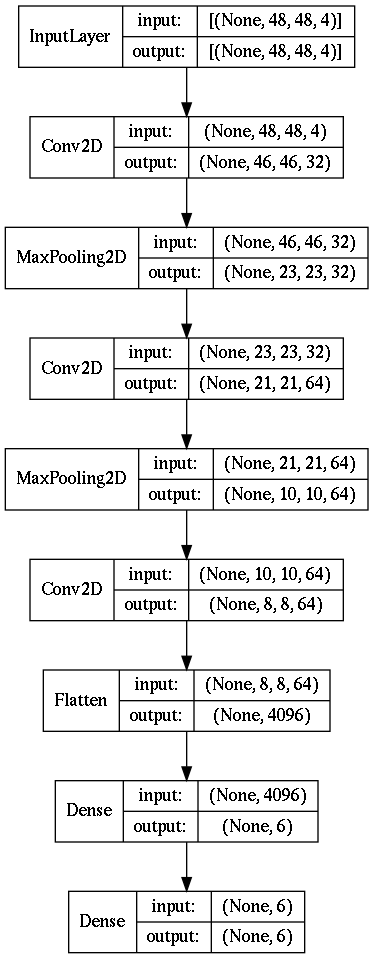
\includegraphics[height=0.9\linewidth]{images/model_cnn.png}
\caption{Basic model for prediction stage}
\label{fig:modelCNN}
\end{figure}

  

        % It's always good to have a results chapter so you can 
        % present how well your ideas and implementations worked
	\chapter{Results}
\label{chap:results}

The learning from basic CNN model at the end of second stage are shown in Fig~\ref{fig:trainCNN} and \ref{fig:trainValCNN}. To improve on this basic CNN model, 81 variants have been tried on less number of iterations (epochs) being under resource constraints \ref{fig:gridSearchCNN10epoch}. As examples in Fig~\ref{fig:example6TP5FN} and \ref{fig:example1FP}, the results from detection stage that classify an object as a car are shown as orange line bounding boxes whereas red dot reveals the ground truth. For reference, A red dot inside bounding box means TP (True Positive), red dot without bounding box means FN (False Negative) and bounding box without any red dot inside means FP (False Positive). There are few cars that have been marked white, these are the masks that were applied to ignore objects that are irrelevant to the problem because of much distance and obstructions in view. CSI Analysis is shown in Figure~\ref{fig:100rowCSI} for the detection stage for YOLO and ResNet (RetinaNet) with different DPT over 100 randomly sampled rows from database.


\begin{figure}
\centering
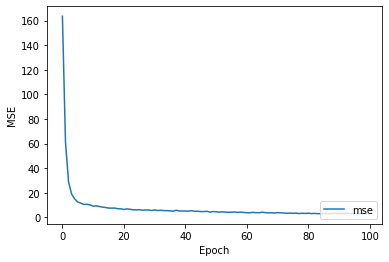
\includegraphics{images/train-1M-data-1000-epoch.png}
\caption{Training learning curve with mean squared error over 1000 epochs}
\label{fig:trainCNN}
\end{figure} 

\begin{figure}
\centering
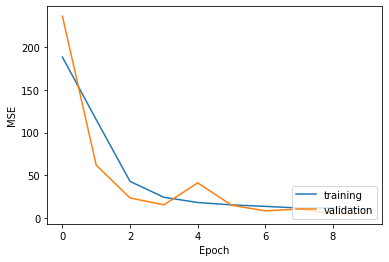
\includegraphics{images/train-val-1M-data-10-epoch.png}
\caption{Training with validation, mean square error over 10 epochs}
\label{fig:trainValCNN}
\end{figure} 

\begin{figure}
\centering
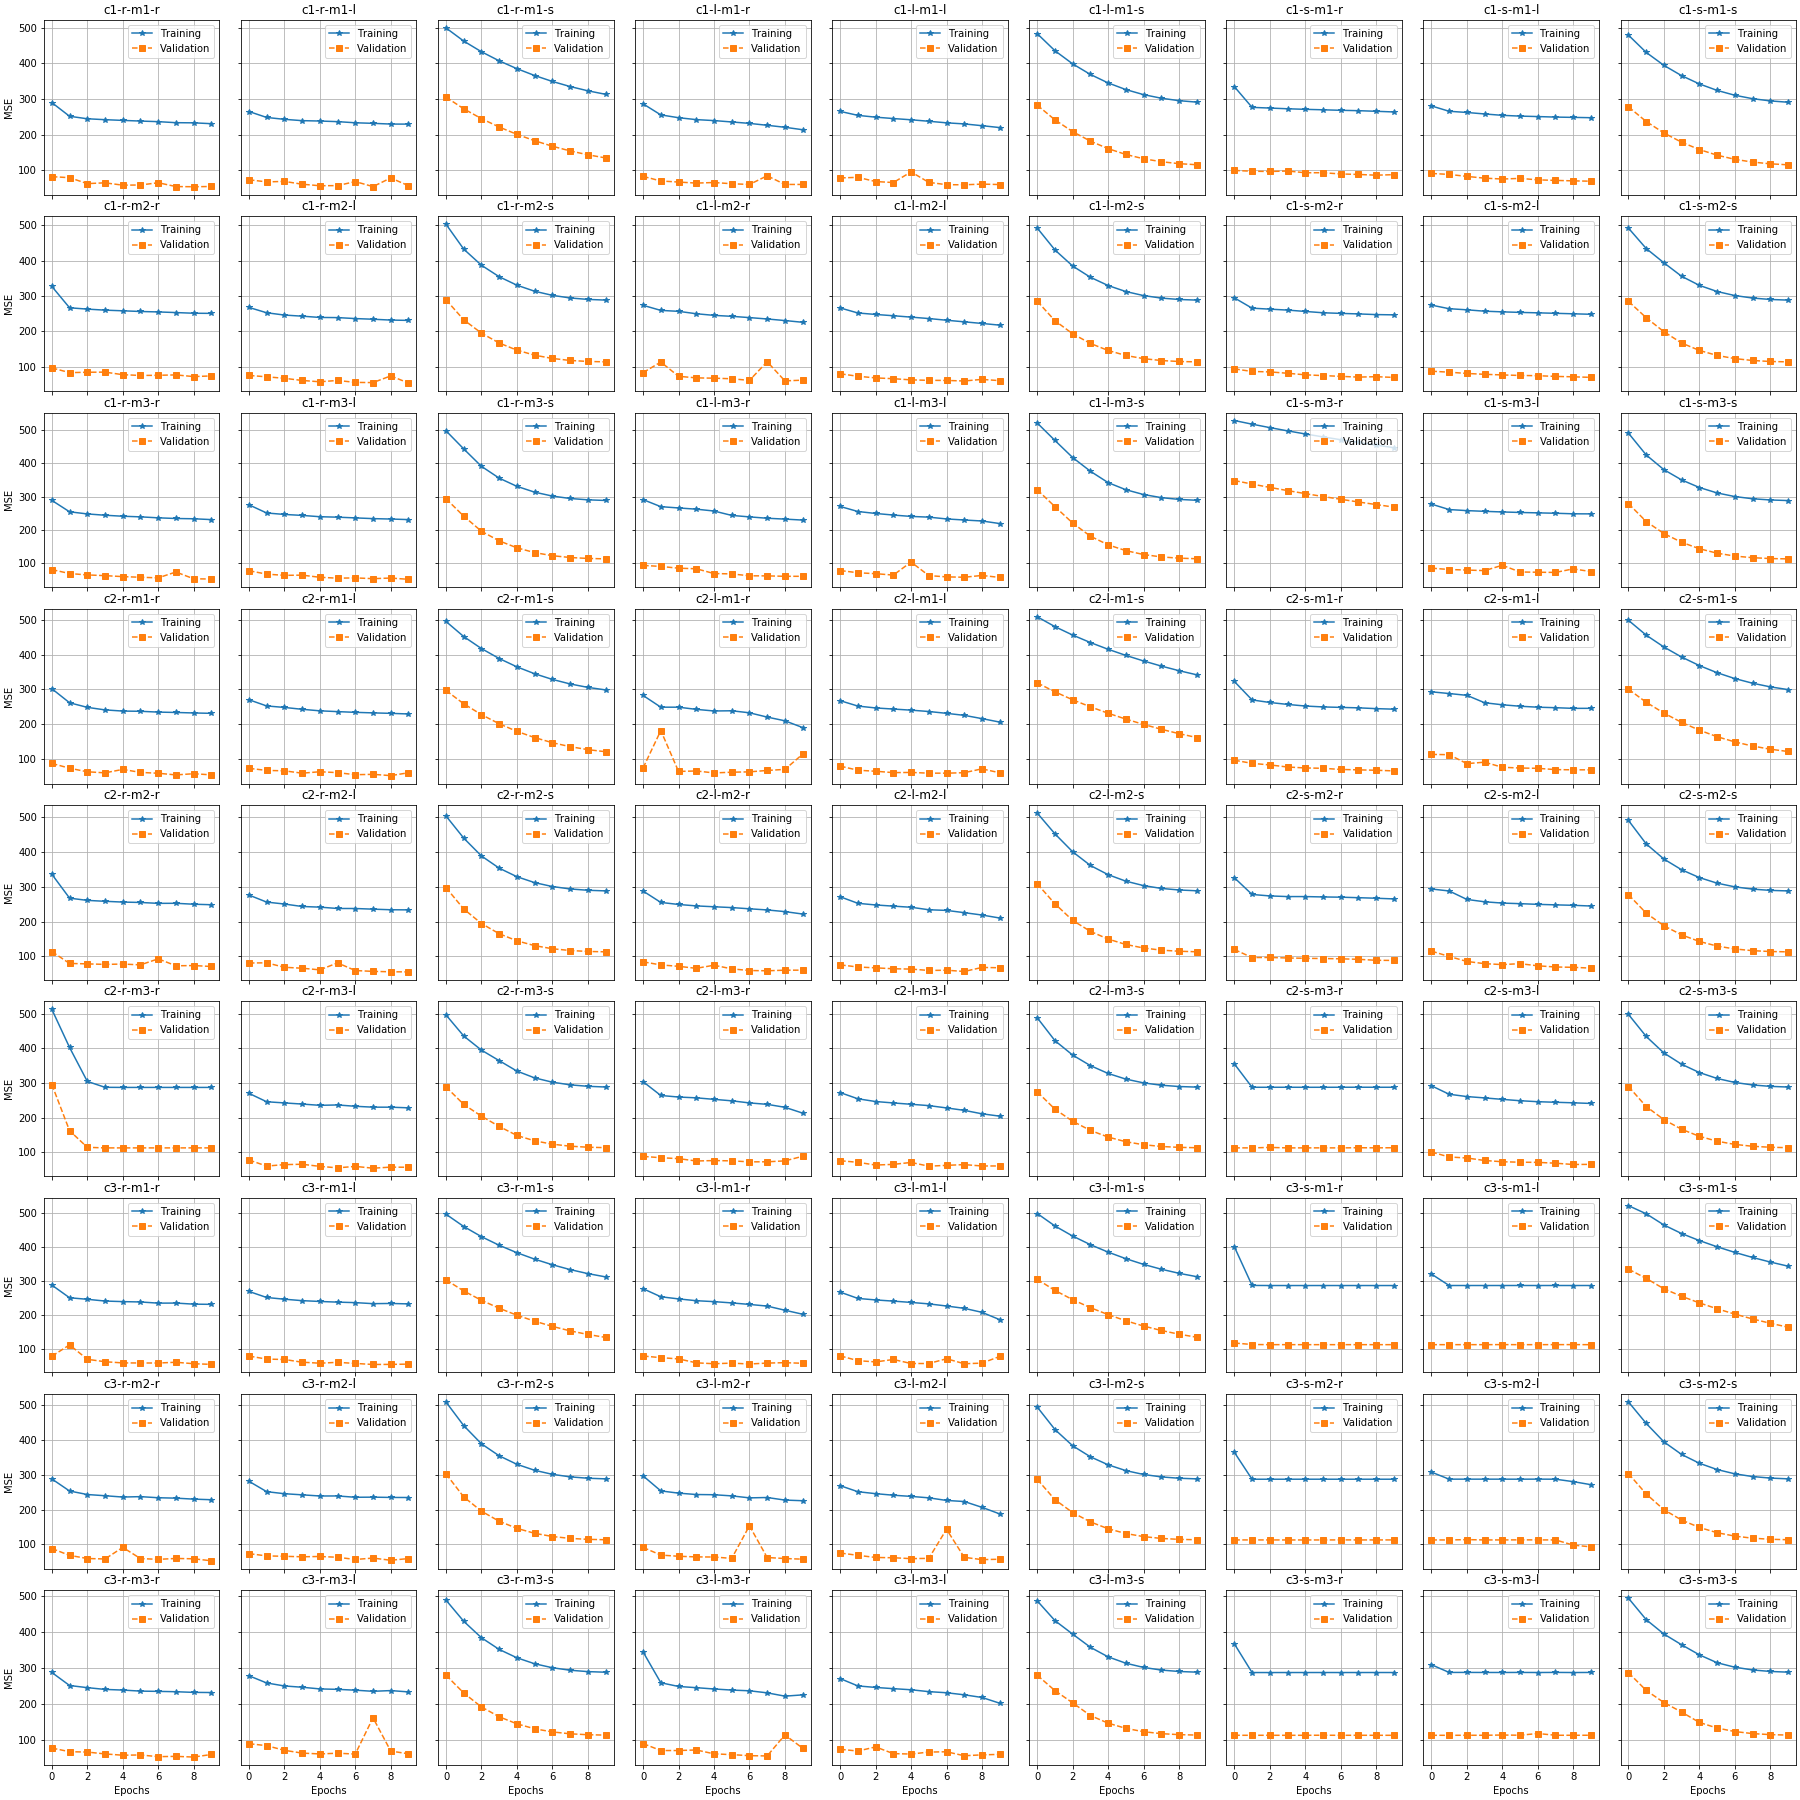
\includegraphics[width=1.0\linewidth]{images/grid-MSE-epochs-10.png}
\caption{CNN model grid search for prediction stage}
\label{fig:gridSearchCNN10epoch}
\end{figure} 


\begin{figure}
\centering
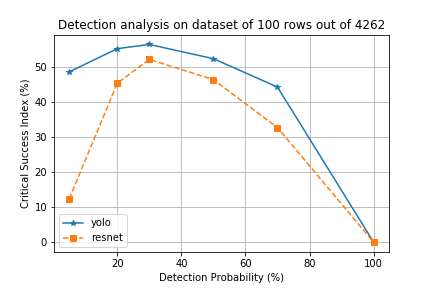
\includegraphics[width=0.8\linewidth]{images/detector_100-rows_CSI-analysis.png}
\caption{CSI analysis for both detection algorithms}
\label{fig:100rowCSI}
\end{figure} 

\begin{figure}
\centering
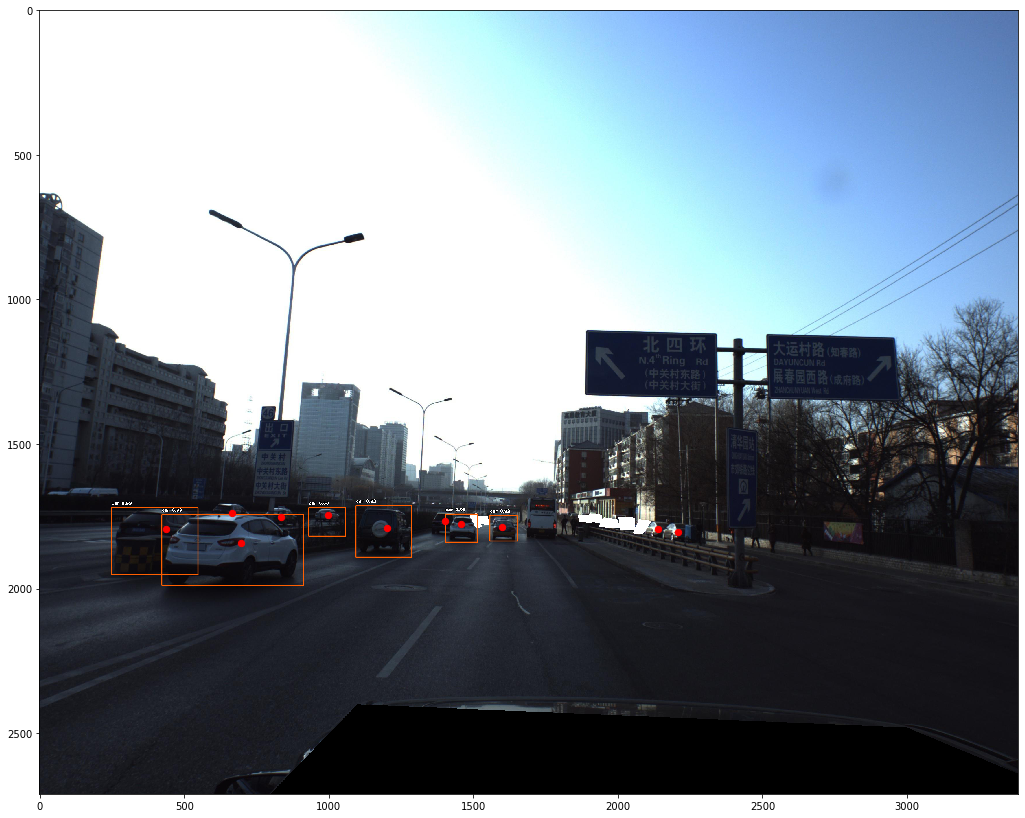
\includegraphics[width=0.8\linewidth]{images/TP-6-FP-0-FN-5.png}
\caption{Detection example 1 - image has 6 TP, 0 FP, 5 FN }
\label{fig:example6TP5FN}
\end{figure} 



\begin{figure}
\centering
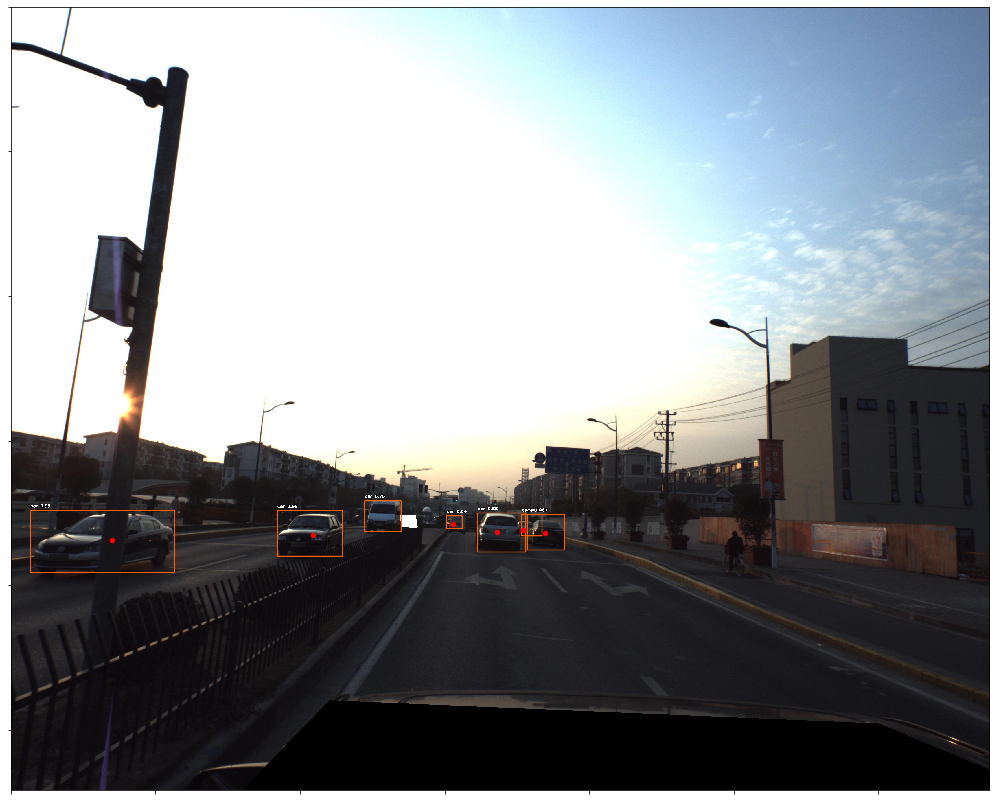
\includegraphics[width=0.8\linewidth]{images/FP-1.png}
\caption{Detection example 2 - image has 1 FP }
\label{fig:example1FP}
\end{figure} 


        % Time to wrap up the thesis with a discussion of your ideas
        % and knowledge that you generated, along with any important
        % insights, or things you learned.  You can include ideas for
        % future extensions and effort here too.
	\chapter{Conclusions and Future Work}
\label{chap:conclusions}

The results need to be combined in a unified metric such as MAP (Mean Average Precision). During training, The predicted angles information can be evaluated against ground truth angles within certain thresholds sorted according to percentage probability feature, to be considered TP (True Positives) and other predictions being FP (False Positives). Precision calculation will then show combined result of two stages and hence degree of relevance of solution to the actual goal.

Second stage also requires many hyper-parameters optimization, such as changing number of hidden layers, number of units in each layer, loss function, activation functions, batch-sizes, longer number of epochs with early stopping etc. 

There is also a possibility of reusing other pre-trained networks for each of the stage.
	
        % If you need an appendix (or appendices), they can be added here 
%	\appendix
\chapter{Appendix A}

Do you need an Appendix?  You can include several of them if you want.

	 
	
        % And finally, don't forget the references and bibliography.
        % You can add entries to the file UMDCS_Thesis.bib for your
        % references.  You then need to ``cite'' them in the tex files
        % by using the ~\cite{ReferenceID} tags.
        %
        % and make sure to include the bib in the TOC
	\newpage
        \printbibliography[heading=bibintoc]
	
\end{document}
